\documentclass[11pt,a4paper,twoside]{book}
\usepackage[utf8]{inputenc}
\usepackage[english]{babel}
\usepackage{amsmath}
\usepackage{amsfonts}
\usepackage{pgfplots}
\usepackage{amssymb}
\usepackage{graphicx}
\author{Ege Özkan}
\title{CENG 422 \\ \large{Design and Managment of Computer Networks Lecture Notes}}
\begin{document}
\newcommand{\unsure}{\textit{?\textsuperscript{*}}}
\newcommand{\missed}{\textit{!\textsuperscript{*}}}
\maketitle
\chapter{Data and Signals - October 20, 2020}
To be transmittedd, data must be transofrmed to electronic signals. Data can be \textit{analog} or it could be \textit{digital}.

\begin{description}
\item[Analog Data] is the information that is continious. It may have a range of infinite values. They tend to be periodic.
\item[Digital Data] is the information that has discrete states. It can only have a limited number of values. They tend to be non-periodic.
\end{description}

\section{Signal Types}

\subsection{Periodic Analog Signals}

Periodic analog signals can be classified as \textit{simple} or \textit{composite}. Two signals may have the same phase and frequency but different amplitudes. The frequency determines the amount of repeats a signal has in a time period.
\begin{figure}
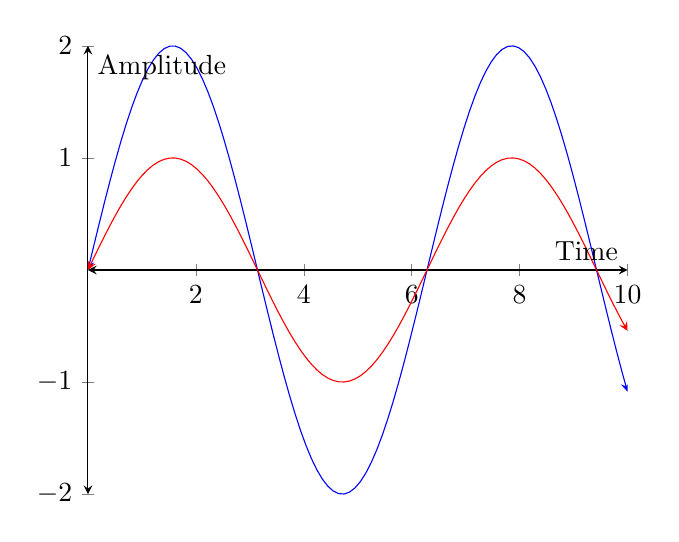
\begin{tikzpicture}[>=stealth]
    \begin{axis}[
        xmin=0,xmax=10,
        ymin=-2,ymax=2,
        axis x line=middle,
        axis y line=middle,
        axis line style=<->,
        xlabel={Time},
        ylabel={Amplitude},
        ]
        \addplot[no marks,blue,<->] expression[domain=0:10,samples=100]{2*sin(deg(x))} 
                    node[pos=0.75,anchor=south west]{};
        \addplot[no marks,red,<->] expression[domain=0:10,samples=100]{sin(deg(x))} 
                    node[pos=0.65,anchor=south west]{}; 
    \end{axis}
\end{tikzpicture}
\caption{Two waves with sample phase and frequency but different amplitude.}
\end{figure}

A period is the amount of time (in seconds) a signal needs to complete 1 cycle, given as $T = \frac{1}{f}$ where $f$ is the frequency.

\begin{figure}
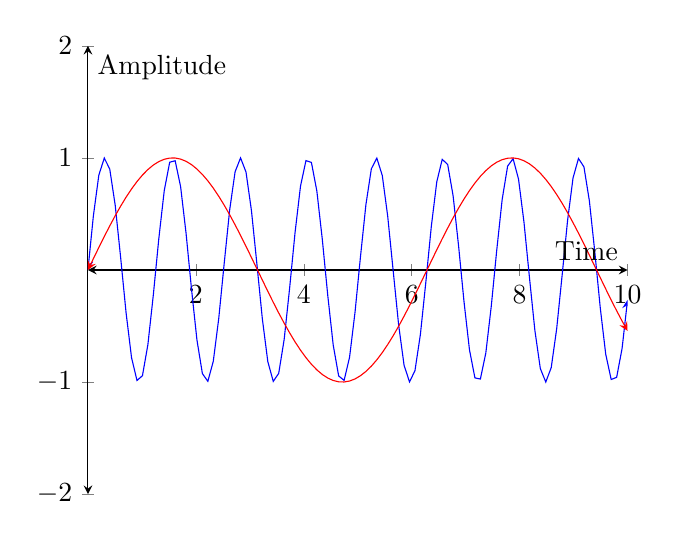
\begin{tikzpicture}[>=stealth]
    \begin{axis}[
        xmin=0,xmax=10,
        ymin=-2,ymax=2,
        axis x line=middle,
        axis y line=middle,
        axis line style=<->,
        xlabel={Time},
        ylabel={Amplitude},
        ]
        \addplot[no marks,blue,<->] expression[domain=0:10,samples=100]{sin(5*deg(x))} 
                    node[pos=0.75,anchor=south west]{};
        \addplot[no marks,red,<->] expression[domain=0:10,samples=100]{sin(deg(x))} 
                    node[pos=0.65,anchor=south west]{}; 
    \end{axis}
\end{tikzpicture}
\caption{Two waves with sample amplitude and phase but different frequency.}
\end{figure}

Frequency is the rate of change with respect to time. Change in a short span of time means high fequency. Otherwise a low frequency. If a frequency does not change at all, its frequency is zero. If the change is instantenious, it is infinite.

\begin{figure}
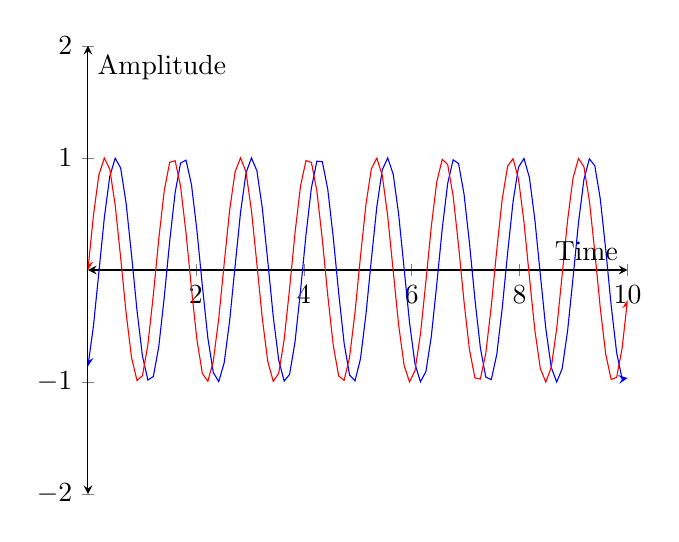
\begin{tikzpicture}[>=stealth]
    \begin{axis}[
        xmin=0,xmax=10,
        ymin=-2,ymax=2,
        axis x line=middle,
        axis y line=middle,
        axis line style=<->,
        xlabel={Time},
        ylabel={Amplitude},
        ]
        \addplot[no marks,blue,<->] expression[domain=0:10,samples=100]{sin(5*deg(x + 1.05))} 
                    node[pos=0.75,anchor=south west]{};
        \addplot[no marks,red,<->] expression[domain=0:10,samples=100]{sin(5*deg(x))} 
                    node[pos=0.65,anchor=south west]{}; 
    \end{axis}
\end{tikzpicture}
\caption{Two waves with sample amplitude and frequency but different phase.}
\end{figure}

The wavelength describes the distance a signal can travel during a period.\\

The waves may be represented using only their frequency domains, simplifying their graphs significantly.

\subsubsection{Composite Signals}

According to Fourier analysis, any composite signal consists of simpler simple signals. If the composite signal is periodic, the decomposition gives a series of signals with discrete frequencies. If the composite signal is nonperiodic, the decomposition gives a combination of sine waves with continuous frequencies.

The \textit{bandwith} of a signal is the difference between the maximum frequency and the minimum frequency it consists of.

\begin{equation}
B = f_h - f_l
\end{equation}

\subsection{Digital Signals}

In digital signals, the amplitude is divided into levels, as the number of levels increase, so does the speed of the transmittion. The \textbf{bitrate} represents the number of bits sent per second. Number of bits that can fit in a number of levels if the number of levels are $n_L$ is:

\begin{equation}
n_B = \log_2 n_L 
\end{equation}

A \textbf{bit length} is the distance that a bit occupies on the transmission medium. Tranmission speed times bitrate.

\begin{equation}
L_B = v \times r_b
\end{equation}

A periodic digital signal occupies an infinite amount of discreate freuqiencies. Whereas non-periodic digital signals (which most of them are.) occupy a continous range of infinite frequencies.\\

\textbf{Baseband transmission} is sending a signal through a channel.

A digital signal necessitates a low-pass channel, a channel that starts from 0Hz.\\

In general, any transmission losses \textit{some} information with regards to the wave form of the signal, to preserve the shape of the signal completely, one needs a low-pass channel with an infinite or very wide bandwith. Sometimes, the digital signal may have to be convert to correspodning analog signals to preserve information.\\

The required bitrate for a bandwith of $b$ is at minimum $\frac{b}{2}$. To acquire better result, once can multiply this number with harmonic sequences.\\

\textbf{Bandpass} is a channel with a limited range of frequencies $f_1 < f < f_2$. A digital signal cannot pass through a bandpass, as it is not a lowpass channel, therefore, the signal is first converted to analog, sent through the channel and then converted back to the digital. These include telephone lines.\\

\section{Tranmission Impairment}

\begin{description}
\item[Attenuation] is the lose of amplitue in the medium, and amplifier can be used to mitigate this issue. The lose and gain can be calculated with the dB unit.
\item[Distortion] Due to the difference of behaviour of the medium for difference frequiences, parts of the composite signal may arrive out of phase, or different.\\
\item[Noise] They may be \textbf{Thermal  Noise} due to the random motiof of electrons in the wire. \textbf{Induced Noise} is noise due to motors or appliences in the environment. \textbf{Crosstalk Noise}, effect of one wire on the other and \textbf{Impulse Noise} is a sudden spike in electricity in the wire. The quality of the medium can be calculated via the SNR (Signal-to-Noise Ratio), higher the SNR, higher the quality of the signal.
\end{description}

\section{Data Rate Limits}

A very important considiration in communication is how fast the data can be sent, in bits per second, over a channel. Keep in mind that, increasing the levels of a signal may reduce the reliability of the system.

\subsection{Formulas}

Maximum data rate of a channel for a noisless channel is the Nyquist formula $L\times n_B \times \log_2 L$ \unsure and for a noisy channel is the Shannon Formula, Capacity $=$ bandwith $+$ $\log_2(1 + \text{SNR})$

\section{Performance}

The bandwith can be calculated in hertz or in bits per second. \textbf{Bandwith delay} is the number of bits that can fit into a channel.
\end{document}